



\subsection{Natural Deduction for Propositional Logic}

\begin{remark}
For this chapter, we replace the word \emph{formula} in rules and 
proofs of a formal system by the word \emph{judgement}.
\end{remark}

\begin{remark}
Judgements in \emph{Natural Deduction} have the form $\Gamma \proofs \varphi$, 
where $\Gamma$ is a set of formulas and $\varphi$ is a formula.
Semantically, $\models \Gamma \proofs \varphi$, i.e., $\Gamma$ derives $\varphi$, meaning that for all interpretations $\valfoo$, if all formulas in $\Gamma$ are true in $\valfoo$, then $\varphi$ is true in $\valfoo$.
Formal system for natural deduction defines a meta-symbol 
$\proofs_\text{meta}$ such that  $\proofs_\text{meta} (\Gamma \proofs 
\varphi)$. 
\end{remark}


\begin{definition}[$\nj$]
    We use the notation $\Gamma, \varphi$ to show $\Gamma \cup \{\varphi\}$. 
    The system \emph{$\nj$} consists of the following rules:
    The axiom introduction
    \begin{center}
    \AxiomC{}
    \RightLabel{\small (ax)}
    \UnaryInfC{$\Gamma, \varphi \proofs \varphi$}
    \DisplayProof
    \end{center}
    The true-introduction, expressing that $\top$ can always be derived, and the false-elimination, expressing if $\bot$ can be derived, then anything can be derived.
    \begin{center}
    \AxiomC{}
    \RightLabel{\small ($\top$-intro)}
    \UnaryInfC{$\Gamma \proofs \top$}
    \DisplayProof
    $\quad$
    \AxiomC{$\Gamma \proofs \bot$}
    \RightLabel{\small ($\bot$-elim)}
    \UnaryInfC{$\Gamma \proofs \varphi$}
    \DisplayProof.
    \end{center}
    Conjunction elimination and introduction
    \begin{center}
    \AxiomC{$\Gamma \proofs \varphi \land \psi$}
    \RightLabel{\small ($\land$-elim)}
    \UnaryInfC{$\Gamma \proofs \varphi$}
    \DisplayProof
    $\quad$
    \AxiomC{$\Gamma \proofs \varphi \land \psi$}
    \RightLabel{\small ($\land$-elim)}
    \UnaryInfC{$\Gamma \proofs \psi$}
    \DisplayProof
    $\quad$
    \AxiomC{$\Gamma \proofs \varphi$}
    \AxiomC{$\Gamma \proofs \psi$}
    \RightLabel{\small ($\land$-intro)}
    \BinaryInfC{$\Gamma \proofs \varphi \land \psi$}
    \DisplayProof.
    \end{center}
     Disjunction elimination and introduction
        \begin{center}
    \AxiomC{$\Gamma \proofs \varphi \lor \psi$}
    \AxiomC{$\Gamma,\varphi \proofs \chi$}
    \AxiomC{$\Gamma, \psi \proofs \chi$}
    \RightLabel{\small ($\lor$-elim)}
    \TrinaryInfC{$\Gamma \proofs \chi$}
    \DisplayProof
    \end{center}
    \begin{center}
    \AxiomC{$\Gamma \proofs \varphi $}
    \RightLabel{\small ($\land$-intro)}
    \UnaryInfC{$\Gamma \proofs \varphi \lor \psi$}
    \DisplayProof
    $\quad$
    \AxiomC{$\Gamma \proofs \psi $}
    \RightLabel{\small ($\land$-intro)}
    \UnaryInfC{$\Gamma \proofs \varphi \lor \psi$}
    \DisplayProof.
    \end{center}
    Negation elimination and introduction
    \begin{center}
    \AxiomC{$\Gamma \proofs \varphi$}
    \AxiomC{$\Gamma \proofs \neg  \varphi$}
    \RightLabel{\small ($\neg$-elim)}
    \BinaryInfC{$\Gamma \proofs \bot$}
    \DisplayProof
    $\quad$
    \AxiomC{$\Gamma , \varphi\proofs \bot $}
    \RightLabel{\small ($\neg$-intro)}
    \UnaryInfC{$\Gamma \proofs \neg \varphi $}
    \DisplayProof.
    \end{center}
    Implication elimination and introduction (observe how $\rightarrow$-elim is similar to modus ponens)
    \begin{center}
    \AxiomC{$\Gamma \proofs \varphi$}
    \AxiomC{$\Gamma \proofs \varphi  \simplies \psi$}
    \RightLabel{\small ($\simplies$-elim)}
    \BinaryInfC{$\Gamma \proofs \psi$}
    \DisplayProof
    $\quad$
    \AxiomC{$\Gamma , \varphi\proofs \psi $}
    \RightLabel{\small ($\simplies$-intro)}
    \UnaryInfC{$\Gamma \proofs \varphi \simplies \psi $}
    \DisplayProof.
    \end{center}
\end{definition}



% \begin{enumerate}
  % \item Axioms
  % \[ \infer* [right=ax]
  %   { }{\Gamma, \varphi \proofs \varphi}
  %   \qquad\qquad \infer* [right=$\top$-intro]
  %   { }{\Gamma \proofs \top}
  % \]
  
  % \item False-elimination: if $\bot$ can be derived, then anything 
  % can be derived.
  % \[ \infer* [right=$\bot$-elim]
  %   {\Gamma \proofs \bot}{\Gamma \proofs \varphi}
  % \]

  % \item Conjunction elimination and introduction
  % \[ \infer* [right=$\land$-elim]
  %   {\Gamma \proofs \varphi \land \psi}{\Gamma \proofs \varphi}
  %   \qquad\qquad \infer* [right=$\land$-elim]
  %   {\Gamma \proofs \varphi \land \psi}{\Gamma \proofs \psi}
  %   \qquad\qquad \infer* [right=$\land$-intro]
  %   {\Gamma \proofs \varphi \\ \Gamma \proofs \psi}
  %   {\Gamma \proofs \varphi \land \psi}
  % \]

  % \item Disjunction elimination and introduction
  % \[ \infer* [right=$\lor$-elim]
  %   {\Gamma \proofs \varphi \lor \psi 
  %   \\ \Gamma, \varphi \proofs \chi
  %   \\ \Gamma, \psi \proofs \chi}{\Gamma \proofs \chi}
  %   \qquad\qquad \infer* [right=$\lor$-intro]
  %   {\Gamma \proofs \varphi}{\Gamma \proofs \varphi \land \psi}
  %   \qquad \infer* [right=$\land$-intro]
  %   {\Gamma \proofs \varphi}{\Gamma \proofs \psi \land \varphi}
  % \]

  % \item Negation elimination and introduction
  % \[ \infer* [right=$\neg$-elim]
  %   {\Gamma \proofs \varphi \\ \Gamma \proofs \neg \varphi}
  %   {\Gamma \proofs \bot}
  %   \qquad\qquad \infer* [right=$\neg$-intro]
  %   {\Gamma, \varphi \proofs \bot}{\Gamma \proofs \neg \varphi}
%   % \]
%   \item Implication elimination and introduction
%   \[ \infer* [right=$\rightarrow$-elim]
%     {\Gamma \proofs \varphi \\ \Gamma \proofs \varphi \rightarrow \psi}
%     {\Gamma \proofs \psi}
%     \qquad\qquad \infer* [right=$\rightarrow$-intro]
%     {\Gamma, \varphi \proofs \psi}{\Gamma \proofs \varphi \rightarrow \psi}
%   \]
  
% \end{enumerate}

\begin{exercise}
      Prove implication transitivity using Natural Deduction.
\end{exercise}



\begin{example}[Contrapositive]
\label{cl7:ex:contrapositive}
  Show $(\varphi \rightarrow \psi) \rightarrow 
  (\neg \psi \rightarrow \neg \varphi)$.
\end{example}
\begin{proof}
We proof this using $\nj$. The proof is represented as a tree and constructed from the root (bottom).

\begin{prooftree}
    \AxiomC{}
    \LeftLabel{\small (ax)}
    \UnaryInfC{$\varphi \simplies \psi, \neg\psi, \varphi \proofs \neg \psi$}
        \AxiomC{}
        \LeftLabel{\small (ax)}
        \UnaryInfC{$\varphi \simplies \psi, \neg\psi, \varphi \proofs \varphi$}
         \AxiomC{}
        \LeftLabel{\small (ax)}
        \UnaryInfC{$\varphi \simplies \psi, \neg\psi, \varphi \proofs \varphi \simplies \psi$}
        \RightLabel{\small($\simplies$-elim)}
        \BinaryInfC{$\varphi \simplies \psi, \neg \psi , \varphi \proofs \psi$}
    \RightLabel{\small($\neg$-elim)}
    \BinaryInfC{$\varphi \simplies \psi, \neg \psi , \varphi \proofs \bot$}
    \RightLabel{\small($\neg$-intro)}
    \UnaryInfC{$\varphi \simplies \psi, \neg \psi \proofs \neg \varphi$}
    \RightLabel{\small($\simplies$-intro)}
    \UnaryInfC{$\varphi \simplies \psi \proofs \neg \psi \simplies \neg \varphi$}
    \RightLabel{\small($\simplies$-intro)}
    \UnaryInfC{$\proofs (\varphi \simplies \psi) \simplies (\neg \psi \simplies \neg \varphi)$}
\end{prooftree}


  % \[ \infer* [right=$\rightarrow$-intro]
  %   { \infer* [right=$\rightarrow$-intro]
  %     { \infer* [right=$\neg$-intro]
  %       { \infer* [right=$\neg$-elim]
  %         { \varphi \rightarrow \psi, \neg \psi, \varphi \proofs \psi \\
  %           \varphi \rightarrow \psi, \neg \psi, \varphi \proofs \neg \psi
  %         }{\varphi \rightarrow \psi, \neg \psi, \varphi \proofs \bot}
  %       }{\varphi \rightarrow \psi, \neg \psi \proofs \neg \varphi}
  %     }{(\varphi \rightarrow \psi) 
  %       \proofs (\neg \psi \rightarrow \neg \varphi)}
  %   }{\proofs (\varphi \rightarrow \psi) 
  %     \rightarrow (\neg \psi \rightarrow \neg \varphi)}
  % \]
  % Now we have two goals to prove. 
  % \[ \infer* [right=$\rightarrow$-elim]
  %   { \infer* [right=ax]
  %     { }{\varphi \rightarrow \psi, \neg \psi, \varphi \proofs \varphi} \\
  %     \infer* [right=ax]
  %     { }{\varphi \rightarrow \psi, \neg \psi, \varphi 
  %         \proofs \varphi \rightarrow \psi}
  %   }{\varphi \rightarrow \psi, \neg \psi, \varphi \proofs \psi}
  %   \qquad \infer* [right=ax]
  %     { }{\varphi \rightarrow \psi, \neg \psi, \varphi \proofs \neg \psi}
  %   \qquad 
  % \]
\end{proof}

\begin{remark}
\label{cl7:rm:box}
Observe how this method of writing proofs in Natural Deduction
requires us to rewrite the context for every step. We can use a
slightly different notation to avoid this repetition.
We can draw boxes to introduce \emph{contexts} in a proof. Every
formula written inside a box is assumed to hold only within that box.
The following ``proofs'' are examples of using this notation.
\[ \infer {
  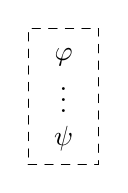
\begin{tikzpicture}
    \node [draw, rectangle, dashed, line cap=round]
    {\begin{tabular}{c} $\varphi$ \\ \vdots \\ $\psi$ \end{tabular}};
  \end{tikzpicture}
  }{\varphi \rightarrow \psi}
  \qquad \infer {
  \begin{tikzpicture}
    \node [draw, rectangle, dashed, line cap=round]
    {\begin{tabular}{c} $\varphi$ \\ \vdots \\ $\bot$ \end{tabular}};
  \end{tikzpicture}
  }{\neg \varphi}
  \qquad \infer {
  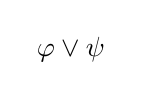
\begin{tikzpicture}
    \node {$\varphi \lor \psi$};
  \end{tikzpicture} \\
  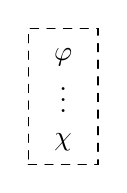
\begin{tikzpicture}
    \node [draw, rectangle, dashed, line cap=round]
    {\begin{tabular}{c} $\varphi$ \\ \vdots \\ $\chi$ \end{tabular}};
  \end{tikzpicture} \\
  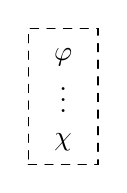
\begin{tikzpicture}
    \node [draw, rectangle, dashed, line cap=round]
    {\begin{tabular}{c} $\varphi$ \\ \vdots \\ $\chi$ \end{tabular}};
  \end{tikzpicture}
  }{\chi}
\]
\end{remark}

\begin{example}
Using the notation from Remark \ref{cl7:rm:box}, we can rewrite the proof for Example
\ref{cl7:ex:contrapositive}:
\[ \infer {
  \begin{tikzpicture}
    \node [draw, rectangle, dashed, line cap=round] {$
    \infer {
      \text{1. } \varphi \rightarrow \psi \\\\
      \begin{tikzpicture}
        \node [draw, rectangle, dashed, line cap=round] {$
        \infer {
          \text{2. } \neg \psi \\\\
          \begin{tikzpicture}
            \node [draw, rectangle, dashed, line cap=round] {
            \begin{tabular}{c}
              3. $\varphi$ \\
              4. $\psi$ ($\rightarrow$-elim, 1, 3) \\
              5. $\bot$ ($\neg$-elim, 2, 4)
            \end{tabular}
            };
          \end{tikzpicture}
        }{\neg \varphi}
        $};
      \end{tikzpicture}
    }{\neg \psi \rightarrow \neg \varphi}
    $};
  \end{tikzpicture}
  }{(\varphi \rightarrow \psi)
    \rightarrow (\neg \psi \rightarrow \neg \varphi)}
\]
\end{example}



\begin{remark}
The system $\nj$ defined is in fact the Intuitionistic Natural 
Deduction system. The following rule, namely the law of excluded
middle, cannot be derived in $\nj$:
\begin{center}
    \AxiomC{}
    \RightLabel{\small (ex)}
    \UnaryInfC{$\Gamma \proofs \varphi \lor  \neg\psi $}
    \DisplayProof.
\end{center}
Assumption of the law of excluded middle is in fact an important
distinction between intuitionistic and classical logic. 
\end{remark}

\begin{definition}[$\nk$]
The system \emph{$\nk$} consists of the same rules as $\nj$ in addition to the law of excluded middle.
\begin{center}
    \AxiomC{}
    \RightLabel{\small (ex)}
    \UnaryInfC{$\Gamma \proofs \varphi \lor  \neg\psi $}
    \DisplayProof.
\end{center}
\end{definition}

\begin{theorem}
The $\nk$ system is sound and complete for propositional logic.
\end{theorem}

\begin{example}
  Show that there exist $a, b \not \in \QN$ such that
  $a ^ b \in \QN$.
\end{example}
\begin{proof}
  Let $a = \sqrt{2} ^ {\sqrt{2}}$ and $b = \sqrt{2}$. We know that
  $\sqrt{2} \not \in \QN$. We do a ``classical''
  case-splitting on $a \in \QN$:
  \begin{itemize}
    \item Case $a \not \in \QN$: We have
    \[ a ^ b
      = \left( \sqrt{2} ^ {\sqrt{2}} \right) ^ {\sqrt{2}}
      = \sqrt{2} ^ 2
      = 2 \in \QN \]
  \item Case $a \in \QN$: We are already done with the proof; let
  $a_1 = b_1 = \sqrt{2}$. We know $a_1, b_1 \not \in \QN$ and,
  by assumption, ${a_1} ^ {b_1} \in \QN$.
  \end{itemize}
  Observe how this classical-style proof utilizes the law of excluded
  middle in the case-splitting: $\sqrt{2} ^ {\sqrt{2}}$ is either in
  $\QN$ or not in $\QN$; there is no \emph{middle}.
\end{proof}



\subsection{Kripke Semantics}

\begin{remark}
Classically, an interpretation $\valfoo\colon P \to \BN$ is defined as a
mapping from a set of propositions to boolean values $\top$ and
$\bot$. For intuitionistic reasoning, we define a new semantics.
\end{remark}

\begin{definition}
  A Kripke model $\kripke$ is defined as a tuple $(W, \krel, w_0,
  \valfoo\colon W \times P \to \BN)$, where $W$ is a set of classical
  worlds, $\krel$ is a pre-order relation on $W$, $w_0$ is the initial
  world, and $\valfoo$ is a function from pairs of world and proposition
  to boolean values such that for any $w, w' \in W$ and any
  $p \in P$, if $w \krel w'$, then $v(w, p) \krel v(w', p)$.
\end{definition}

\begin{remark}
Informally, a Kripke model is an interpretation model for
intuitionistic proof systems. 
\end{remark}

\begin{theorem}
    The following facts hold for any Kripke
model $m$: (i)  $\kripke \models \varphi$ iff $m \proofs_{w_0} \varphi$;
(ii) $\kripke\not \models_w \bot$ for any world $w$; (iii) $\kripke \models_w p$ iff $\valfoo(w, p) = \top$; (iv) $\kripke \models_w \varphi \rightarrow \psi$ iff for any $w'$, if $w \krel w'$ and $\kripke \models_{w'} \varphi$, then $\kripke \models_{w'} \psi$.
\end{theorem}

\begin{remark}
  In $\nj$, whenever you show $\varphi \lor \psi$, you need to show either
$\varphi$, or $\psi$. As previously stated, the law of excluded middle
cannot be derived in $\nj$. To show this, we need to show that there
exists a Kripke model $\kripke$ such that excluded middle is false in a
world $w$ of $\kripke$.  
\end{remark}


\begin{example}
Let us define a Kripke model with only one proposition $p$ and only
two worlds $w_0$ and $w_1$, where $w_0 \krel w_1$, and $p$ is false in
$w_0$ and true in $w_1$.
\begin{center}
  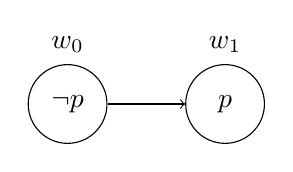
\begin{tikzpicture}
    \node (w0) at (0, 0) [draw, circle,  minimum size=1cm] {$\neg p$};
    \node (w1) at (2, 0) [draw, circle,  minimum size=1cm] {$p$};
    \node at (0, .75) {$w_0$};
    \node at (2, .75) {$w_1$};
    \draw[->] (w0) -- (w1);
  \end{tikzpicture}
\end{center}
Let us examine what formulas are true (or false) in each world. By
definition, $p$ is false in $w_0$. Let us examine the value of
$\neg p$ in $w_0$. We can safely substitute $\neg p$ with $p
\simplies \bot$. By definition, $p \simplies \bot$ holds in
$w_0$ iff for any world $w$, if $w_0 \krel w$ and $p$ is true in $w$,
then $\bot$ is true in $w$. We know $p$ is true in $w_1$. We also
know that $\bot$ is not true in $w_1$, as it is not true in any world.
So, by definition, $p \simplies \bot$ is false in $w_0$. So, both
$p$ and $\neg p$ are false in $w_0$, from which we obtain that $p
\lor \neg p$ is also false in $w_0$.
\end{example}


\subsection{Sequent (Gentzen) Calculus and $\lk$}

\begin{remark}
Judgements in the $\lk$ proof system have the form $\Gamma \proofs
\Delta$, where both $\Gamma$ and $\Delta$ are sets of formulas.
Judgement $\Gamma \proofs \Delta$ should be read as ``the
\emph{conjunction} of the formulas in $\Gamma$ implies the
\emph{disjunction} of the formulas in $\Delta$''. Semantically, for
a classical interpretation $\valfoo$, $\valfoo \models (\Gamma \proofs \Delta)$
if and only if, if all formulas in $\Gamma$ are true under $\valfoo$, then
some formula in $\Delta$ is true under $\valfoo$.
\end{remark}


\begin{definition}
    The Sequent (Gentzen) Calculus is composed of the following rules. 
    (Observe how every non-axiom judgement increases the number of logical
    connectives in the set of formulas.)
    Axioms 
    \begin{center}
      \AxiomC{}
      \RightLabel{\small (ax)}
      \UnaryInfC{$\Gamma, \varphi \proofs \varphi, \Delta$}
      \DisplayProof
      $\quad$
      \AxiomC{}
      \RightLabel{\small $\bot$-elim}
      \UnaryInfC{$\Gamma, \bot \proofs \Delta$}
      \DisplayProof
      $\quad$
      \AxiomC{}
      \RightLabel{\small  $\top$-intro}
      \UnaryInfC{$\Gamma \proofs \top, \Delta$}
      \DisplayProof
    \end{center}
    Conjunction
    \begin{center}
      \AxiomC{$\Gamma, \varphi, \psi \vdash \Delta$}
      \RightLabel{\small($\land$-left)}
      \UnaryInfC{$\Gamma, \varphi \land \psi \vdash \Delta$}
      \DisplayProof
      $\quad$
    \AxiomC{$\Gamma \vdash \varphi, \Delta$}
      \AxiomC{$\Gamma \vdash \psi, \Delta$}
      \RightLabel{\small($\land$-right)}
      \BinaryInfC{$\Gamma \vdash \varphi \land \psi, \Delta$}
      \DisplayProof
      $\quad$
    \end{center}
    Disjunction
    \begin{center}
      \AxiomC{$\Gamma, \varphi \vdash \Delta$}
      \AxiomC{$\Gamma, \psi \vdash \Delta$}
      \RightLabel{\small($\lor$-left)}
      \BinaryInfC{$\Gamma, \varphi \lor \psi \vdash \Delta$}
      \DisplayProof
      $\quad$
      \AxiomC{$\Gamma \vdash \varphi, \psi, \Delta$}
      \RightLabel{\small($\lor$-right)}
      \UnaryInfC{$\Gamma \vdash \varphi \lor \psi, \Delta$}
    \DisplayProof
    \end{center}
    Negation
    \begin{center}
         \AxiomC{$\Gamma, \varphi \vdash \Delta$}
      \RightLabel{$\neg$-right}
      \UnaryInfC{$\Gamma \vdash \neg \varphi, \Delta$}
      \DisplayProof
      $\quad$
       \AxiomC{$\Gamma \vdash \varphi, \Delta$}
      \RightLabel{$\neg$-left}
      \UnaryInfC{$\Gamma, \neg \varphi \vdash \Delta$}
      \DisplayProof
    \end{center}
     Implication
         \begin{center}
  \AxiomC{$\Gamma, \varphi \vdash \psi, \Delta$}
      \RightLabel{$\rightarrow$-right}
      \UnaryInfC{$\Gamma \vdash \varphi \rightarrow \psi, \Delta$}
      \DisplayProof
      $\quad$
      \AxiomC{$\Gamma \vdash \varphi, \Delta$}
      \AxiomC{$\Gamma, \psi \vdash \Delta$}
      \RightLabel{$\rightarrow$-left}
      \BinaryInfC{$\Gamma, \varphi \rightarrow \psi \vdash \Delta$}
      \DisplayProof
    \end{center}
\end{definition}


% \begin{enumerate}
%   \item 
%   \item Conjunction
%   \[ \infer
%     {\Gamma, \varphi, \psi \proofs \Delta}
%     {\Gamma, \varphi \land \psi \proofs \Delta}
%     \qquad\qquad \infer
%     {\Gamma \proofs \varphi, \Delta
%     \\ \Gamma \proofs \psi, \Delta}
%     {\Gamma \proofs \varphi \land \psi, \Delta}
%   \]
%   \item Disjunction
%   \[ \infer
%     {\Gamma, \varphi \proofs \Delta
%     \\ \Gamma, \psi \proofs \Delta}
%     {\Gamma, \varphi \lor \psi \proofs \Delta}
%     \qquad\qquad \infer
%     {\Gamma \proofs \varphi, \psi, \Delta}
%     {\Gamma \proofs \varphi \lor \psi, \Delta}
%   \]
%   \item Negation
%   \[ \infer
%     {\Gamma, \varphi \proofs \Delta}
%     {\Gamma \proofs \neg \varphi, \Delta}
%     \qquad\qquad \infer
%     {\Gamma \proofs \varphi, \Delta}
%     {\Gamma, \neg \varphi \proofs \Delta}
%   \]
%   \item Implication
%   \[ \infer
%     {\Gamma, \varphi \proofs \psi, \Delta}
%     {\Gamma \proofs \varphi \rightarrow \psi, \Delta}
%     \qquad\qquad \infer
%     {\Gamma \proofs \varphi, \Delta
%     \\ \Gamma, \psi \proofs \Delta}
%     {\Gamma, \varphi \rightarrow \psi \proofs \Delta}
%   \]
% \end{enumerate}

\begin{theorem}
    The $\lk$ proof system is sound and complete for propositional logic.
This actually means that excluded middle can be derived in $\lk$.
\end{theorem}


\begin{exercise}
  Prove the following in $\lk$: (i) The law of excluded middle: $ \proofs p \lor \neg p$ and (ii) implication transitivity.
\end{exercise}
